\documentclass{beamer}
% This is the file main.tex

\usetheme{AIP}

\newsavebox{\longestsec}% Box to save longest sectional heading


\pgfdeclareimage[width = 0.50\paperwidth]{big}{cos}% insert fancy image for entertainment
\title{The SCAN project: First results}% your talk title 
\author[Arman]{Arman Khalatyan }% Full Name of speaker 
\institute[AIP]{Leibniz Institute for Astrophysics Potsdam}% institute keep it as it is. 
\date{\today}
%fine tuning for sections 
\AtBeginSection[]
{
  \begin{frame}<beamer>
    \frametitle{Outline for section \thesection}
    \tableofcontents[currentsection]
  \end{frame}
}

\begin{document}

\begin{frame}
\titlepage
\end{frame}

\begin{frame}
  \frametitle{Table of contents}
  \tableofcontents
\end{frame}



\section{Introduction}
\subsection{Motivation}
\begin{frame}
\frametitle{Motivation}
Why? \alert{target...}
\end{frame}
\subsection{Algorithms}
\begin{frame}
\frametitle{Algorithms}
\begin{itemize}
\item Isodensity finder
\item Density estimation
\end{itemize}
\subsection{The Data}
\end{frame}
\section{The Data}
\begin{frame}
\frametitle{Cosmology}
\begin{description}[Second Item]
\item[WMAP7] Many snapshots from CLUES
\item[CURIE] Some SFR simulation from Gustavo
\item[Ugly vs GOOD] Testing differences between Cosmologies 
\end{description}
\end{frame}
\section{Results}
\begin{frame}[t]
\frametitle{Filemetns, Sheets and more}
Nice rendering from \textit{PMViewer}
\begin{figure}
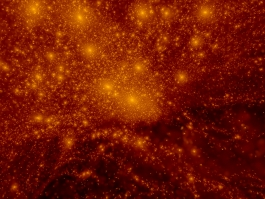
\includegraphics[width = 0.50\paperwidth]{a} 
\caption{show an example picture}
\end{figure}
\end{frame}



\end{document}
